% !TeX program = pdfLaTeX
\documentclass[12pt]{article}
\usepackage{amsmath}
\usepackage{graphicx,psfrag,epsf}
\usepackage{enumerate}
\usepackage{natbib}
\usepackage{textcomp}
\usepackage[hyphens]{url} % not crucial - just used below for the URL
\usepackage{hyperref}

%\pdfminorversion=4
% NOTE: To produce blinded version, replace "0" with "1" below.
\newcommand{\blind}{0}

% DON'T change margins - should be 1 inch all around.
\addtolength{\oddsidemargin}{-.5in}%
\addtolength{\evensidemargin}{-.5in}%
\addtolength{\textwidth}{1in}%
\addtolength{\textheight}{1.3in}%
\addtolength{\topmargin}{-.8in}%

%% load any required packages here



% tightlist command for lists without linebreak
\providecommand{\tightlist}{%
  \setlength{\itemsep}{0pt}\setlength{\parskip}{0pt}}



\usepackage[dvipsnames]{xcolor} % colors
\newcommand{\ear}[1]{{\textcolor{blue}{#1}}}
\newcommand{\svp}[1]{{\textcolor{RedOrange}{#1}}}
\newcommand{\rh}[1]{{\textcolor{Green}{#1}}}
\usepackage[capitalise]{cleveref}
\newcommand\pcref[1]{(\cref{#1})}
\usepackage{algorithm,algpseudocode,booktabs}

\begin{document}


\def\spacingset#1{\renewcommand{\baselinestretch}%
{#1}\small\normalsize} \spacingset{1}


%%%%%%%%%%%%%%%%%%%%%%%%%%%%%%%%%%%%%%%%%%%%%%%%%%%%%%%%%%%%%%%%%%%%%%%%%%%%%%

\if0\blind
{
  \title{\bf Eye Fitting Straight Lines in the Modern Era}

  \author{
        Emily A. Robinson 1 \\
    Department of Statistics, University of Nebraska - Lincoln\\
     and \\     Reka Howard 2 \\
    Department of Statistics, University of Nebraska - Lincoln\\
     and \\     Susan VanderPlas 3 \\
    Department of Statistics, University of Nebraska - Lincoln\\
      }
  \maketitle
} \fi

\if1\blind
{
  \bigskip
  \bigskip
  \bigskip
  \begin{center}
    {\LARGE\bf Eye Fitting Straight Lines in the Modern Era}
  \end{center}
  \medskip
} \fi

\bigskip
\begin{abstract}
How do statistical regression results compare to intuitive, visually
fitted results? Fitting lines by eye through a set of points has been
explored since the 20th century. Common methods of fitting trends by eye
involve maneuvering a string, black thread, or ruler until the fit is
suitable, then drawing the line through the set of points. In 2015, the
New York Times introduced an interactive feature, called `You Draw It',
where readers were asked to input their own assumptions about various
metrics and compare how these assumptions relate to reality. In this
paper, we validate `You Draw It' as a method for graphical testing,
comparing results to the less technological method utilized in
\citet{mosteller1981eye} and extending that study with formal
statistical analysis methods. Results were consistent with those found
in the previous study; when shown points following a linear trend,
participants tended to fit the slope of the first principal component
over the slope of the least-squares regression line. This trend was most
prominent when shown data simulated with larger variances. This study
reinforces the differences between intuitive visual model fitting and
statistical model fitting, providing information about human perception
as it relates to the use of statistical graphics.
\end{abstract}

\noindent%
{\it Keywords:} Cognitive Bias, Graph Perception, Graphical
Testing, Linear Regression, Statistical Graphics, Visualization
\vfill

\newpage
\spacingset{1.45} % DON'T change the spacing!

\hypertarget{introduction}{%
\section{Introduction}\label{introduction}}

We all use statistical graphics, but how do we know that the graphics we
use are communicating properly? When creating a graphic, we must
consider the design choices most effective for conveying the intended
result. For instance, we may decide to highlight the relationship
between two variables in a scatter-plot by including a trend line, or
adding color to highlight clustering \citep{vanderplas2017clusters}.
These design choices require that we understand the perceptual and
visual biases that come into play when creating graphics, and as
graphics are evaluated visually, we must use human testing to ground our
understanding in empiricism.

Much of the research on the perception of visual features in charts has
been conducted in psychophysics and tests for accuracy and quantitative
comparisons when understanding a plot. \citet{cleveland1984graphical}
conducted a series of cognitive tasks designed to establish a hierarchy
of visual components for making comparisons. For example, it is more
effective to display information on an \(x\) or \(y\) axis rather than
using color in order to reduce the visual effort necessary to make
numerical comparisons. \citet{cleveland1985graphical} found that
assessing the position of points along an axis is easier than
determining the slope of a line. Other studies focus on the viewers
ability to perceive the strength of the relationship between \(x\) and
\(y\) coordinates in a scatter-plot. For instance, when the data appear
dense, viewers tend to overestimate the magnitude of the correlation
coefficient \citep{cleveland1982variables, lauer1989density}.
\citet{cleveland1993visualizing} provides an argument for displaying
cyclical patterns with an aspect ratio which sets the curve close to
45\(^{\circ}\). \citet{kosslyn2006graph} examines how Gestalt principles
of perceptual organization are instrumental in extracting data from a
chart. For example, data points that are closer in space are more likely
to be perceived as grouped \citep{ciccione2020grouping}, and vertical
and horizontal lines are easier to discriminate than oblique ones
\citep{appelle1972perception}. The results of these cognitive tasks
provide some consistent guidance for chart design; however, other
methods of visual testing can further evaluate design choices and help
us understand cognitive biases related to the evaluation of statistical
charts.

\hypertarget{testing-statistical-graphics}{%
\subsection{Testing Statistical
Graphics}\label{testing-statistical-graphics}}

We need human testing of graphics in order to draw broad conclusions,
develop guidelines for graphical design, and improve graphical
communication. Studies might ask participants to identify differences in
graphs, read information off of a chart accurately, use data to make
correct real-world decisions, or predict the next few observations. All
of these types of tests require different levels of use and manipulation
of the information being presented in the chart. Early research studies
considered graphs from a psychological perspective
\citep{spence1990visual, lewandowsky1989perception}, testing
participants' abilities to detect a stimulus or a difference between two
stimuli. Psychophysical methods have been used to test graphical
perception, as in \citet{vanderplas2015signs}, which used the method of
adjustment to estimate the magnitude of the impact of the sine illusion.
However, there are more modern testing methods that have been developed
since the heyday of psychophysics.

One major development in statistical graphics which led to more advanced
testing methods is Wilkinson's Grammar of Graphics
\citep{wilkinson2013grammar}. The grammar of graphics serves as the
fundamental framework for data visualization with the notion that
graphics are built from the ground up by specifying exactly how to
create a particular graph from a given data set. Visual representations
are constructed through the use of ``tidy data'' which is characterized
as a data set in which each variable is in its own column, each
observation is in its own row, and each value is in its own cell
\citep{wickham2016r}. Graphics are viewed as a mapping from variables in
a data set (or statistics computed from the data) to visual attributes
such as the axes, colors, shapes, or facets on the canvas in which the
chart is displayed. Software, such as Hadley Wickham's ggplot2
\citep{wickham2011ggplot2}, aims to implement the framework of creating
charts and graphics as the grammar of graphics recommends.

Combining the grammar of graphics with another tool for statistical
graphics testing, the statistical lineup, yields a method for evaluating
graphical design choices. \citet{buja2009statistical} introduced the
lineup protocol to provide a framework for inferential testing. Through
experimentation, methods such as the lineup protocol allow researchers
to conduct studies geared at understanding human ability to conduct
tasks related to the perception of statistical charts such as
differentiation, prediction, estimation, and extrapolation
\citep{vanderplas2017clusters, vanderplas2015spatial, hofmann2012graphical}.
The advancement of graphing software provides the tools necessary to
develop new methods of testing statistical graphics.

While these testing methods are excellent, there is one particular
subset of statistical graphics testing methods which we intend to
develop further in this paper: assessing graphics by fitting statistical
models ``by eye''.

\hypertarget{fitting-trends-by-eye}{%
\subsection{Fitting Trends by Eye}\label{fitting-trends-by-eye}}

Initial studies in the 20th century explored the use of fitting lines by
eye through a set of points
\citep{finney1951subjective, mosteller1981eye}. Common methods of
fitting trends by eye involved maneuvering a string, black thread, or
ruler until the fit is suitable, then drawing the line through the set
of points. Recently, \citet{ciccione2021can} conducted a comprehensive
set of studies investigating human ability to detect trends in graphical
representations using physical adjustment and manipulation methods.

\citet{finney1951subjective} used graphical testing for computational
purposes: to determine the effect of stopping iterative maximum
likelihood calculations after one iteration. Many techniques in
statistical analysis are performed with the aid of iterative
calculations such as Newton's method or Fisher's scoring. The author was
interested in whether one iteration of calculations was sufficient in
the estimation of parameters connected with pharmaceutical dose-response
relationships. In pharmaceuticals, one measure of interest is the
relative potency between a test preparation of doses and standard
preparation of does; relative potency is calculated as the ratio of two
equally effective doses between the two preparation methods. In this
study, twenty-one scientists were recruited via postal mail and asked to
``rule two lines'' in order to judge by eye the positions for a pair of
parallel probit regression lines in a biological assay. The author then
computed one iterative calculation of the relative potency based on
starting values as determined by the pair of lines drawn by each
participant. The author then compared these relative potency estimates
to that which was estimated by the full probit technique (reaching
convergence through multiple iterations). Results of the study indicated
that one cycle of iterations for calculating the relative potency was
sufficient based on the starting values provided by eye from the
participants.

\citet{mosteller1981eye} sought to understand the properties of least
squares and other computed lines by establishing one systematic method
of fitting lines by eye. Participants were asked to fit lines by eye to
four scatter-plots using an 8.5 x 11 inch transparency with a straight
line etched completely across the middle. A latin square design with
packets of the set of points stapled together in four different
sequences was used to determine if there is an effect of order of
presentation. It was found that order of presentation had no effect and
that participants tended to fit the slope of the principal axis (error
minimized orthogonally, both horizontal and vertical, to the regression
line) over the slope of the least squares regression line (error
minimized vertically to the regression line). These results support
previous research on ``ensemble perception'' indicating the visual
system can compute averages of various features in parallel across the
items in a set
\citep{chong2003representation, chong2005statistical, van2011rapid}.

In \citet{ciccione2021can}, participants were asked to judge trends,
estimate slopes, and conduct extrapolation. To estimate slopes,
participants were asked to report the slope of the best-fitting
regression line using a track-pad to adjust the tilt of a line on the
screen. Results indicated the slopes participants reported were always
in excess of the ideal slopes, both in the positive and in the negative
direction, and those biases increase with noise and with number of
points. This supports the results found in \citet{mosteller1981eye} and
suggest that participants might use Deming regression
\citep{deming1943statistical, linnet1998performance, martin2000general},
which minimizes the Euclidean distance of points from the line, when
fitting a line to a noisy scatter-plot.

While not explicitly intended for perceptual testing, in 2015, the New
York Times introduced an interactive feature, called You Draw It
\citep{aisch_cox_quealy_2015, buchanan_park_pearce_2017, katz_2017}.
Readers were asked to input their own assumptions about various metrics
and compare how these assumptions relate to reality. The New York Times
team utilizes Data Driven Documents (D3) \citep{bostock2011d3} that
allows readers to predict these metrics through the use of drawing a
line on their computer screen with their computer mouse. After the
reader has completed drawing the line, the actual observed values are
revealed and the reader may check their estimated knowledge against the
actual reported data. While this interactive feature is designed to get
readers to confront their own intuitions about data in the news, we feel
that the interactivity of this method may be useful for the purpose of
graphical testing and measuring the patterns humans see in data.

In this paper, we establish `You Draw It', adapted from the New York
Times feature, as a tool for graphical testing. Our visual system is
naturally built to look for structure and identify patterns. For
instance, points going down from left to right indicates a negative
correlation between the x and y variables. Our research is intended to
implement the `You Draw It' feature as a way to measure the patterns we
see in data. We validate the `You Draw It' method by replicating the
less technological study conducted by \citet{mosteller1981eye}. Based on
previous research surrounding ``ensemble perception,'' we hypothesize
that visual regression tends to mimic principle component regression
rather than an ordinary least squares regression. In order to assess
this hypothesis, we introduce a method for statistically modeling the
participant drawn lines using generalized additive mixed models.

\hypertarget{methods}{%
\section{Methods}\label{methods}}

\hypertarget{participants}{%
\subsection{Participants}\label{participants}}

Participants were recruited through through Twitter, Reddit, and direct
email in May 2021. A total of 35 individuals completed 119 unique `You
Draw It' task plots; data collected from all completed `You Draw It'
task plots were included in the analysis. All participants had normal or
corrected to normal vision and signed an informed consent form. The
experimental tasks took approximately 15 minutes to complete. While this
study does utilize a convenience sample, as this is primarily a
perceptual task, previous results have found few differences between
expert and non-expert participants in this context
\citep{vanderplas2015spatial}. These data were collected to validate
this method of graphical testing, with the hopes of providing a new tool
to assess graphical perception interactively. Participants completed the
experiment on their own computers in an environment of their choosing.
The experiment was conducted and distributed through a Shiny application
\citep{shinyPkg} found
\href{https://emily-robinson.shinyapps.io/you-draw-it-validation-applet/}{here}.

\hypertarget{you-draw-it-task}{%
\subsection{`You Draw It' Task}\label{you-draw-it-task}}

In the study, participants were shown an interactive scatter-plot
(\cref{fig:ydi-stimuli}) along with the prompt, ``Use your mouse to fill
in the trend in the yellow box region.'' The yellow box region moves
along as the user draws their trend-line, providing a visual cue which
indicates where the user still needs to complete a trend line. After the
entire domain has been visually estimated or predicted, the yellow
shaded region disappears, indicating the participant has completed the
task. Data Driven Documents (D3), a JavaScript-based graphing framework
that facilitates user interaction, is used to create the `You Draw It'
visual. In order to allow for user interaction and data collection, we
integrated the D3 visual into Shiny using the \texttt{r2d3} package.
While the interface is highly customized to this particular task, we
hope to generalize the code and provide a Shiny widget in an R package
soon.

\begin{figure}[tbp]

{\centering 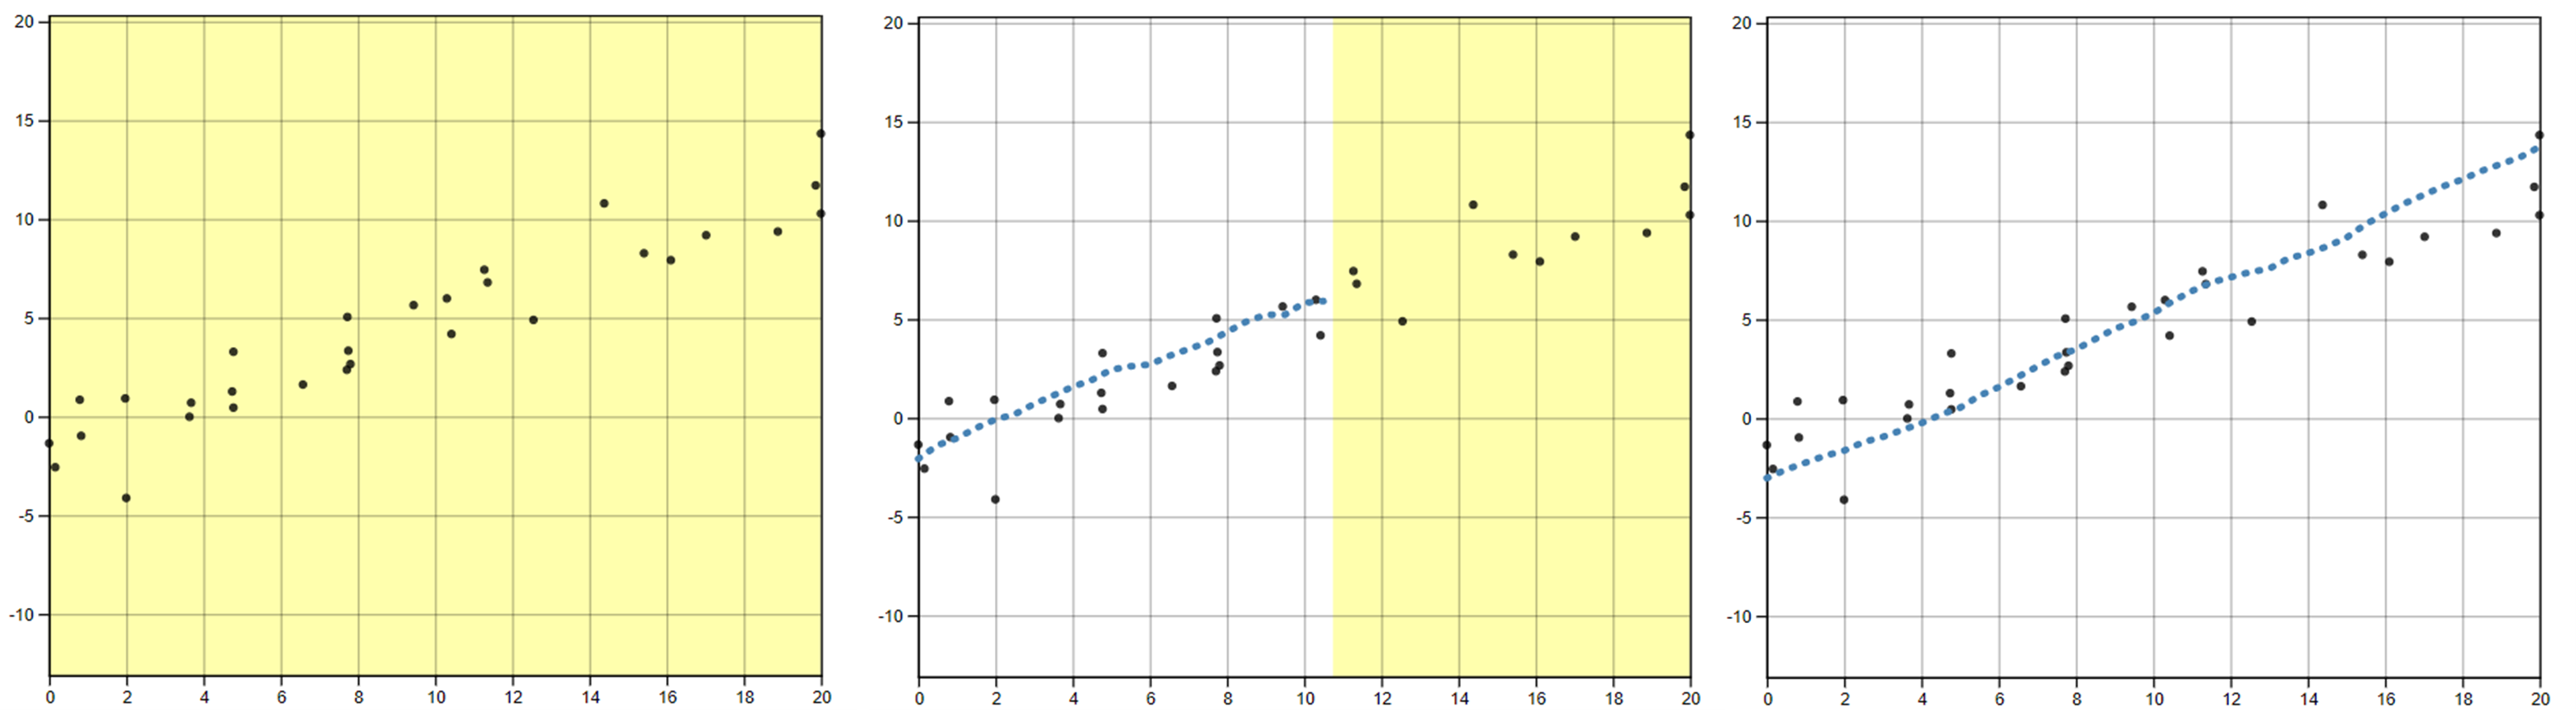
\includegraphics[width=1\linewidth,]{images/ydi-stimuli} 

}

\caption{'You Draw It' task plot as shown to particpants during the study. The first frame (left) illustrates what particpants first see with the prompt “Use your mouse to fill in the trend in the yellow box region.” The second frame (middle), illustrates what the particpant sees while completing the task; the yellow shaded region provides a visual cue for participants indicating where the participant still needs to complete a trend-line. The last frame (right) illustrates the participants finished trend-line before submission.}\label{fig:ydi-stimuli}
\end{figure}

\hypertarget{data-generation}{%
\subsection{Data Generation}\label{data-generation}}

All data processing was conducted in R statistical software. A total of
\(N = 30\) points \((x_i, y_i), i = 1,...N\) were generated for
\(x_i \in [x_{min}, x_{max}]\) where \(x\) and \(y\) have a linear
relationship. Data were simulated based on a linear model with additive
errors: \begin{align}
y_i & = \beta_0 + \beta_1 x_i + e_i \\
\text{with } e_i & \sim N(0, \sigma^2). \nonumber
\end{align}

Model equation parameters, \(\beta_0\) and \(\beta_1\), were selected to
reflect the four data sets (F, N, S, and V) used in
\citet{mosteller1981eye} (\cref{tab:eyefitting-parameters}). We obtain
\(\beta_0\) from the point-slope equation of a line using the mean of
the generated \(x\) values and the predefined \(y\) value at \(\bar x\),
denoted \(y_{\bar x}\). Parameter choices F, N, and S simulated data
across a domain of 0 to 20. Parameter choice F produces a trend with a
positive slope and a large variance while N has a negative slope and a
large variance. In comparison, S shows a trend with a positive slope
with a small variance and V yields a steep positive slope with a small
variance over the domain of 4 to 16. \cref{fig:eyefitting-simplot}
illustrates an example of simulated data for all four parameter choices
intended to reflect the trends in \citet{mosteller1981eye}. Aesthetic
design choices were made consistent across each of the interactive `You
Draw It' task plots. The y-axis range extended 10\% beyond (above and
below) the range of the simulated data points to allow for users to draw
outside the simulated data set range and avoid anchoring their lines to
the corners of the plot.

\begin{table}

\caption{\label{tab:eyefitting-parameters}Designated model equation parameters for simulated data.}
\centering
\begin{tabular}[t]{cccc}
\toprule
Parameter Choice & $y_{\bar{x}}$ & $\beta_1$ & $\sigma$\\
\midrule
S & 3.88 & 0.66 & 1.30\\
F & 3.90 & 0.66 & 1.98\\
V & 3.89 & 1.98 & 1.50\\
N & 4.11 & -0.70 & 2.50\\
\bottomrule
\end{tabular}
\end{table}

\begin{figure}[tbp]

{\centering 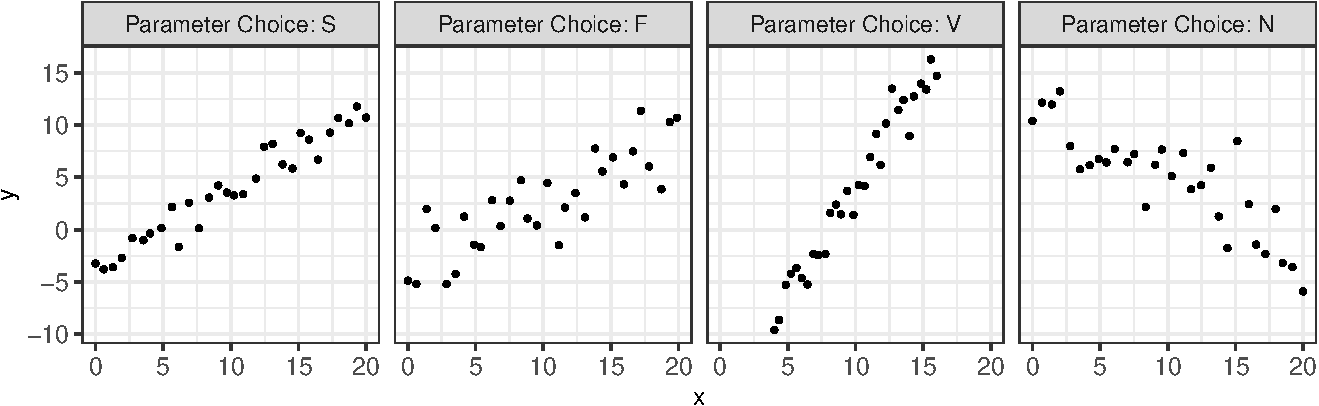
\includegraphics[width=1\linewidth,]{Eye-Fitting-Straight-Lines-in-the-Modern-Era_files/figure-latex/eyefitting-simplot-1} 

}

\caption{Example of simulated data points displayed in a scatter-plot illustrating the trends associated with the four selected parameter choices.}\label{fig:eyefitting-simplot}
\end{figure}

\hypertarget{study-design}{%
\subsection{Study Design}\label{study-design}}

This experiment was conducted as part of a larger study of the
perception of log and linear scales; for simplicity, we focused on the
study design and methods related to the current study. Each scatter-plot
was the graphical representation of a data set that was generated
randomly and independently for each participant at the start of the
experiment. Participants in the study were shown two `You Draw It'
practice plots in order to train participants in the skills associated
with executing the task - in particular, the responsiveness of the
applet requires that participants draw a line at a certain speed,
ensuring that all of the evenly spaced points along the hand-drawn line
are filled in. During the practice session, participants were provided
with instruction prompts accompanied by a .gif and a practice plot.
Instructions guided participants to start at the edge of the yellow box,
to make sure the yellow shaded region is moving along with their mouse
as they draw, and that they can draw over their already drawn line.
Practice plots were then followed by four `You Draw It' task plots
associated with the current study. The order of the task plots was
randomly assigned for each individual in a completely randomized design.

\hypertarget{results}{%
\section{Results}\label{results}}

\hypertarget{fitted-regression-lines}{%
\subsection{Fitted Regression Lines}\label{fitted-regression-lines}}

We compare the participant drawn line to two regression lines determined
by ordinary least squares (OLS) regression and regression based on the
principal axis (PCA). \cref{fig:ols-vs-pca-example} illustrates the
difference between an OLS regression line which minimizes the vertical
distance of points from the line and a regression line based on the
principal axis which minimizes the Euclidean distance of points
(orthogonal) from the line.

Due to the randomness in the data generation process, the actual slope
of the linear regression line fit through the simulated points could
differ from the predetermined slope. Therefore, we fit an OLS regression
to each scatter-plot to obtain estimated parameters
\(\hat\beta_{0,OLS}\) and \(\hat\beta_{1,OLS}\). Fitted values,
\(\hat y_{k,OLS}\), were then obtained every 0.25 increments across the
domain from the OLS regression equation,
\(\hat y_{k,OLS} = \hat\beta_{0,OLS} + \hat\beta_{1,OLS} x_k\)., for
\(k = 1, ..., 4 x_{max} +1\). The regression equation based on the
principal axis was determined by using the \texttt{princomp} function in
the stats package in base R to obtain the rotation of the coordinate
axes from the first principal component (direction which captures the
most variance). The estimated slope, \(\hat\beta_{1,PCA}\), is
determined by the ratio of the axis rotation in \(y\) and axis rotation
in \(x\) of the first principal component with the y-intercept,
\(\hat\beta_{0,PCA}\) calculated by the point-slope equation of a line
using the mean of the simulated points, \((\bar x_i, \bar y_i)\). Fitted
values, \(\hat y_{k,PCA}\), were then obtained every 0.25 increment
across the domain from the PCA regression equation,
\(\hat y_{k,PCA} = \hat\beta_{0,PCA} + \hat\beta_{1,PCA} x_k\).

\begin{figure}[tbp]

{\centering 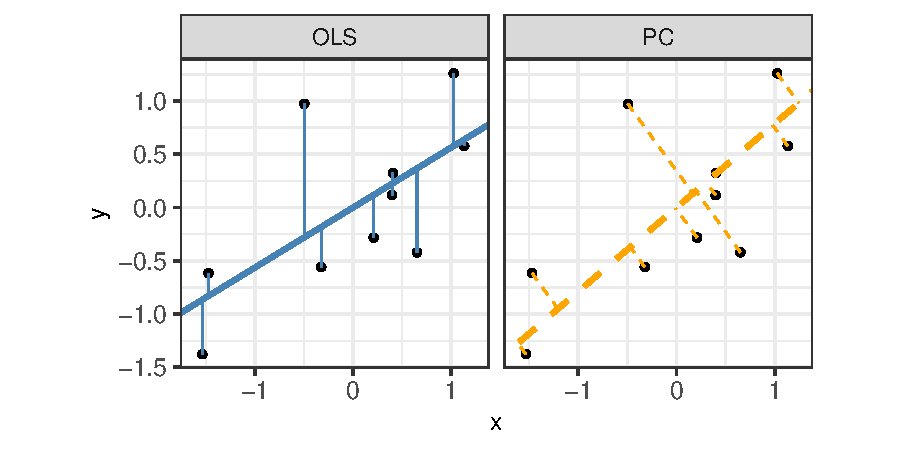
\includegraphics[width=0.8\linewidth,]{Eye-Fitting-Straight-Lines-in-the-Modern-Era_files/figure-latex/ols-vs-pca-example-1} 

}

\caption{ Comparison between an OLS regression line which minimizes the vertical distance of points from the line and a regression line based on the principal axis which minimizes the Euclidean distance of points (orthogonal) from the line.}\label{fig:ols-vs-pca-example}
\end{figure}

\hypertarget{residual-trends}{%
\subsection{Residual Trends}\label{residual-trends}}

For each participant, the final data set used for analysis contained
\(x_{ijk}, y_{ijk,drawn}, \hat y_{ijk,OLS}\), and \(\hat y_{ijk,PCA}\)
for parameter choice \(i = 1,2,3,4\), j = \(1,...N_{participant}\), and
\(x_{ijk}\) value for increment \(k = 1, ...,4 x_{max} + 1\). Using both
a linear mixed model and a generalized additive mixed model, comparisons
of vertical residuals in relation to the OLS fitted values
(\(e_{ijk,OLS} = y_{ijk,drawn} - \hat y_{ijk,OLS}\)) and PCA fitted
values (\(e_{ijk,PCA} = y_{ijk,drawn} - \hat y_{ijk,PCA}\)) were made
across the domain. \cref{fig:eyefitting-example-plot} displays an
example of all three fitted trend lines for parameter choice F.

\begin{figure}[tbp]

{\centering 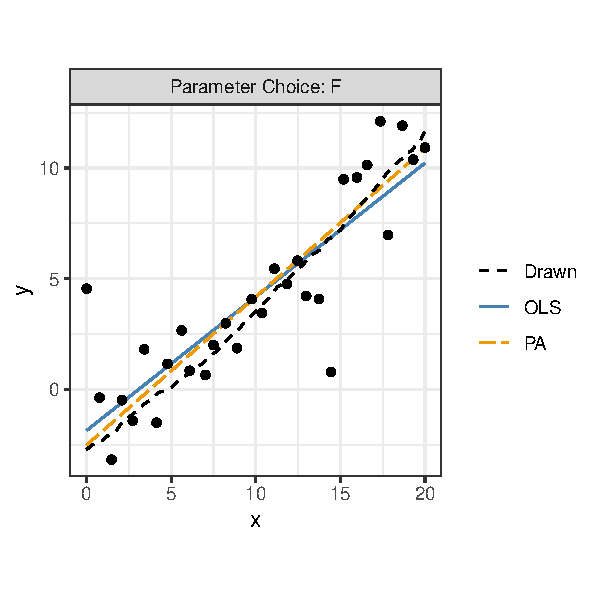
\includegraphics[width=0.5\linewidth,]{Eye-Fitting-Straight-Lines-in-the-Modern-Era_files/figure-latex/eyefitting-example-plot-1} 

}

\caption{Illustrates the data associated with and collected for one `You Draw It' task plot. Trend-lines include the participant drawn line (dashed black), the OLS regression line (solid steelblue) and the PCA regression line based on the principal axis (solid orange).}\label{fig:eyefitting-example-plot}
\end{figure}

\hypertarget{linear-trend-constraint}{%
\subsubsection{Linear Trend Constraint}\label{linear-trend-constraint}}

Using the \texttt{lmer} function in the lme4 package \citep{lme4}, a
linear mixed model (LMM) is fit separately to the OLS residuals and PCA
residuals, constraining the fit to a linear trend. Parameter choice,
\(x\), and the interaction between \(x\) and the parameter choice were
treated as fixed effects with a random participant effect accounting for
variation due to participant. The LMM equation for each fit (OLS and
PCA) is given by: \begin{equation}
y_{ijk,drawn} - \hat y_{ijk,fit} = e_{ijk,fit} = \left[\gamma_0 + \alpha_i\right] + \left[\gamma_{1} x_{ijk} + \gamma_{2i} x_{ijk}\right] + p_{j} + \epsilon_{ijk}
\end{equation} \noindent where

\begin{itemize}
\tightlist
\item
  \(y_{ijk,drawn}\) is the drawn \(y\) value for the \(i^{th}\)
  parameter choice, \(j^{th}\) participant, and \(k^{th}\) increment of
  \(x\) value
\item
  \(\hat y_{ijk,fit}\) is the fitted \(y\) value for the \(i^{th}\)
  parameter choice, \(j^{th}\) participant, and \(k^{th}\) increment of
  \(x\) value corresponding to either the OLS or PCA fit
\item
  \(e_{ijk,fit}\) is the residual between the drawn and fitted \(y\)
  values for the \(i^{th}\) parameter choice, \(j^{th}\) participant,
  and \(k^{th}\) increment of \(x\) value corresponding to either the
  OLS or PCA fit
\item
  \(\gamma_0\) is the overall intercept
\item
  \(\alpha_i\) is the effect of the \(i^{th}\) parameter choice (F, S,
  V, N) on the intercept
\item
  \(\gamma_1\) is the overall slope for \(x\)
\item
  \(\gamma_{2i}\) is the effect of the parameter choice on the slope
\item
  \(x_{ijk}\) is the \(x\) value for the \(i^{th}\) parameter choice,
  \(j^{th}\) participant, and \(k^{th}\) increment
\item
  \(p_{j} \sim N(0, \sigma^2_{participant})\) is the random error due to
  the \(j^{th}\) participant's characteristics
\item
  \(\epsilon_{ijk} \sim N(0, \sigma^2)\) is the residual error.
\end{itemize}

Constraining the residual trend to a linear fit,
\cref{fig:eyefitting-lmer-residualplots} shows the estimated trend line
of the residuals between the participant drawn points and fitted values
for both the OLS regression line and PCA regression line. Estimated
residual trend lines are overlaid on the observed individual participant
residuals. Results indicate the estimated trends of PCA residuals
(orange) appear to align closer to the \(y=0\) horizontal (dashed) line
than the OLS residuals (blue). In particular, this trend is more
prominent in parameter choices with large variances (F and N). These
results are consistent to those found in \citet{mosteller1981eye}
indicating participants fit a trend-line closer to the estimated
regression line with a slope based on the first principal axis than the
estimated OLS regression line thus, providing support for ``ensemble
perception''.

\begin{figure}[tbp]

{\centering 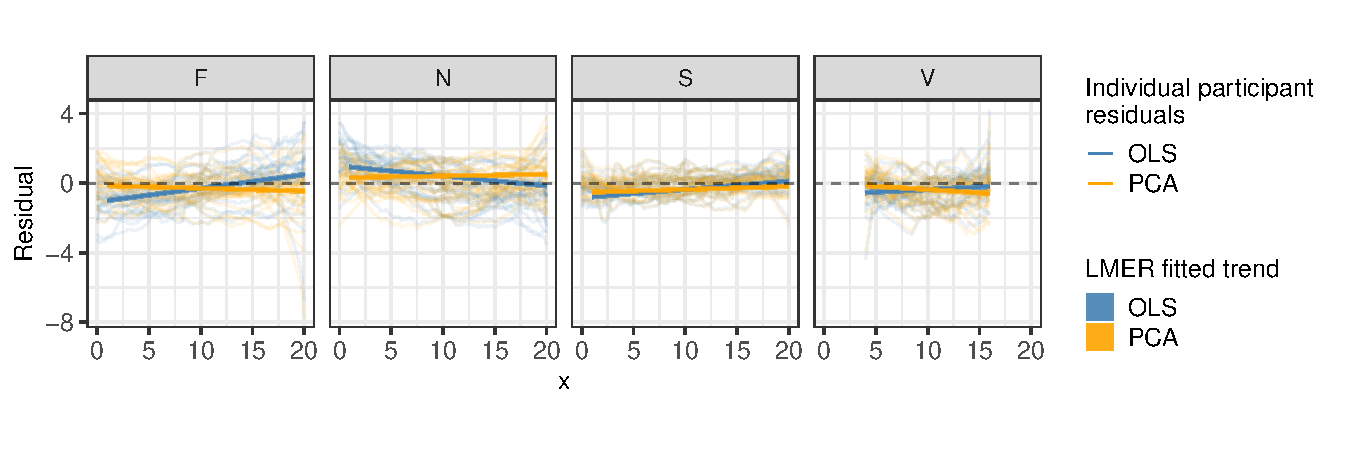
\includegraphics[width=1\linewidth,]{Eye-Fitting-Straight-Lines-in-the-Modern-Era_files/figure-latex/eyefitting-lmer-residualplots-1} 

}

\caption{Estimated trend line of the residuals between the participant drawn points and fitted values for both the OLS (blue) regression line and PCA (orange) regression line constrained to a linear fit modeled by a linear mixed model. Estimated residual trends with 95\% confidence bands are overlaid on the observed individual participant residuals.}\label{fig:eyefitting-lmer-residualplots}
\end{figure}

\hypertarget{smoothing-spline-trend}{%
\subsubsection{Smoothing Spline Trend}\label{smoothing-spline-trend}}

Eliminating the linear trend constraint, the \texttt{bam} function in
the mgcv package \citep{mgcv1, mgcv2, mgcv3, mgcv4, mgcv5} is used to
fit a generalized additive mixed model (GAMM) separately to the OLS
residuals and PCA residuals to allow for estimation of smoothing
splines. Parameter choice was treated as a fixed effect with no
estimated intercept and a separate smoothing spline for \(x\) was
estimated for each parameter choice. A random participant effect
accounting for variation due to participant and a random spline for each
participant accounted for variation in spline for each participant. The
GAMM equation for each fit (OLS and PCA) residuals is given by:
\begin{equation}
y_{ijk, drawn} - \hat y_{ijk, fit} = e_{ijk,fit} = \alpha_i + s_{i}(x_{ijk}) + p_{j} + s_{j}(x_{ijk})
\end{equation} \noindent where

\begin{itemize}
\tightlist
\item
  \(y_{ijk,drawn}\) is the drawn \(y\) value for the \(i^{th}\)
  parameter choice, \(j^{th}\) participant, and \(k^{th}\) increment of
  \(x\) value
\item
  \(\hat y_{ijk,fit}\) is the fitted \(y\) value for the \(i^{th}\)
  parameter choice, \(j^{th}\) participant, and \(k^{th}\) increment of
  \(x\) value corresponding to either the OLS or PCA fit
\item
  \(e_{ijk,fit}\) is the residual between the drawn and fitted \(y\)
  values for the \(i^{th}\) parameter choice, \(j^{th}\) participant,
  and \(k^{th}\) increment of \(x\) value corresponding to either the
  OLS or PCA fit
\item
  \(\alpha_i\) is the intercept for the parameter choice \(i\)
\item
  \(s_{i}\) is the smoothing spline for the \(i^{th}\) parameter choice
\item
  \(x_{ijk}\) is the \(x\) value for the \(i^{th}\) parameter choice,
  \(j^{th}\) participant, and \(k^{th}\) increment
\item
  \(p_{j} \sim N(0, \sigma^2_{participant})\) is the error due to
  participant variation
\item
  \(s_{j}\) is the random smoothing spline for each participant.
\end{itemize}

Allowing for flexibility in the residual trend,
\cref{fig:eyefitting-gamm-residualplots} shows the estimated trend line
of the residuals between the participant drawn points and fitted values
for both the OLS regression line and PCA regression line. Estimated
residual trends were overlaid on the observed individual participant
residuals. The results of the GAMM align with those shown in
\cref{fig:eyefitting-lmer-residualplots} providing support that for
scatter-plots with more noise (F and N), estimated trends of PCA
residuals (orange) appear to align closer to the \(y=0\) horizontal
(dashed) line than the OLS residuals (blue). By fitting smoothing
splines, we can determine whether participants naturally fit a straight
trend-line to the set of points or whether they deviate throughout the
domain. In particular, in scatter-plots with smaller variance (S and V),
we can see that participants began at approximately the correct starting
point then deviated away from the fitted regression lines and corrected
for their fit toward the end of their trend-line. In scatter-plots with
larger variance (F and N), participants estimated their starting value
in the extreme direction of the OLS regression line based on the
increasing or decreasing trend but more accurately represented the
starting value of the PCA regression line. As participants continued
their trend-line, they crossed through the OLS regression line
indicating they estimated the slope in the extreme direction. These
results provide further insight into the curvature humans perceive in a
set of points.

\begin{figure}[tbp]

{\centering 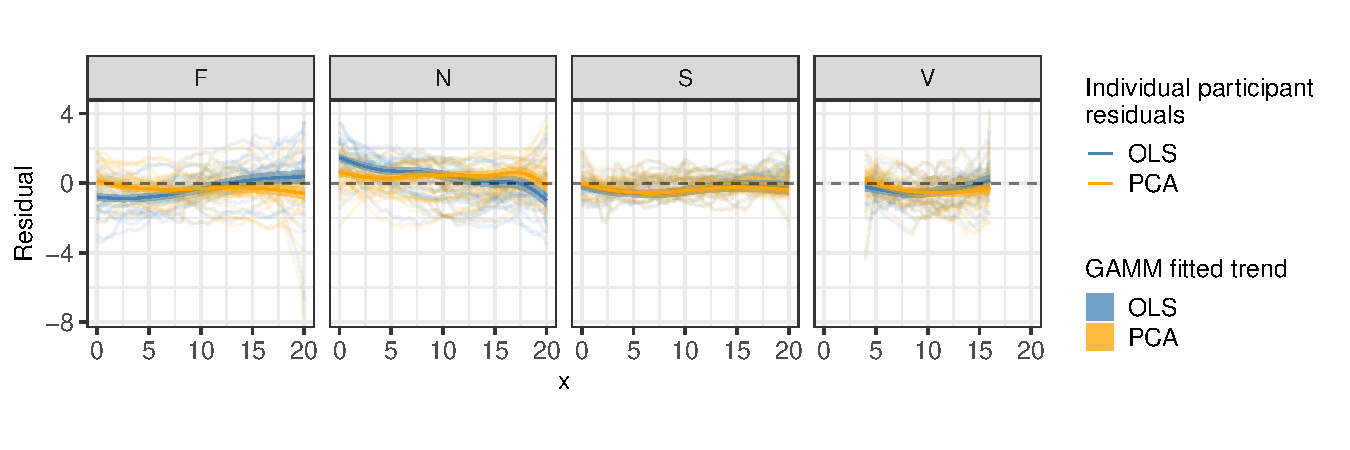
\includegraphics[width=1\linewidth,]{Eye-Fitting-Straight-Lines-in-the-Modern-Era_files/figure-latex/eyefitting-gamm-residualplots-1} 

}

\caption{Estimated trend line of the residuals between the participant drawn points and fitted values for both the OLS (blue) regression line and PCA (orange) regression line determined by smoothing splines fit by a generalized additive mixed model. Estimated residual trends with 95\% confidence bands are overlaid on the observed individual participant residuals.}\label{fig:eyefitting-gamm-residualplots}
\end{figure}

\hypertarget{discussion-and-conclusion}{%
\section{Discussion and Conclusion}\label{discussion-and-conclusion}}

The intent of this research was to adapt `You Draw It' from the New York
Times feature as a tool and method for testing graphics and introduce a
method for statistically modeling the participant drawn lines. We
provided support for the validity of the `You Draw It' method by
replicating the study found in \citet{mosteller1981eye}. Using
generalized additive mixed models, we assessed the deviation of the
participant drawn lines from the statistically fitted regression lines.
Our results found that when shown points following a linear trend,
participants visually fit a regression line that mimics the first
principle component regression as opposed to ordinary least squares
regression. Data simulated with a larger variance provided strong
support for a participants tendency to visually fit the first principle
component regression. Our results indicate that participants minimized
the distance from their drawn regression line over both the \(x\) and
\(y\) axis simultaneously. We utilized modern technology to replicate a
study conducted 40 years ago, and strengthened the original results with
current analysis methods which allow for more flexibility and
sophistication. These results provide support that humans perform
``ensemble perception'' in a statistical graphic setting. We allowed
participants to draw trend lines that deviated from a straight line and
gained an insight into the curvature the human eye perceives in a set of
points.

\hypertarget{future-work}{%
\section{Future Work}\label{future-work}}

This study provided a basis for the use of `You Draw It' as a tool for
testing statistical graphics and introduced a method for statistically
modeling participant drawn lines using generalized additive mixed
models. Further investigation is necessary to implement this method in
non-linear settings and with real data in order to facilitate scientific
communication. This tool could also be used to evaluate human ability to
extrapolate data from trends. In the future, we intend to create an R
package designed for easy implementation of `You Draw It' task plots in
order to make this tool accessible to other researchers.

\newpage
\begin{center}
{\large\bf SUPPLEMENTARY MATERIAL}
\end{center}

\begin{itemize}
\tightlist
\item
  \textbf{Participant Data:} De-identified participant data collected in
  the study and used for analyses are available to be downloaded from
  GitHub
  \href{https://github.com/earobinson95/Eye-Fitting-Straight-Lines-in-the-Modern-Era/tree/main/data}{here}.
\item
  \textbf{Data Analysis Code:} The code used to replicate the analysis
  in this paper can be found
  \href{https://earobinson95.github.io/Eye-Fitting-Straight-Lines-in-the-Modern-Era/analysis/you-draw-it-eyefitting-analysis.html}{here}.
\item
  \textbf{Study Applet:} The shiny app used to conduct the study can be
  accessed
  \href{https://emily-robinson.shinyapps.io/you-draw-it-validation-applet/}{here}.
\item
  \textbf{RShiny Applet Code:} The code used to create the RShiny Applet
  for data collection can be found
  \href{https://github.com/earobinson95/you-draw-it-validation-applet}{here}.
\end{itemize}

\bibliographystyle{agsm}
\bibliography{bibliography.bib}


\end{document}
